%% ============================================================================
%% PAPER_HOTMOBILE_6PG.tex — the 6-page HotMobile 2027 submission. (2026-08-17)
%%
%% WHY THIS FILE EXISTS ALONGSIDE THE LONG DRAFTS. PAPER_HOTMOBILE_2027.tex holds
%% ~13,300 words + 6 figures + 6 tables ≈ 3x the venue's hard limit (6 pages
%% INCLUDING references; deadline 2026-10-09). The CFP explicitly favors "early
%% work and papers likely to stimulate reflection and discussion over a '6-pages
%% conference paper'" — the long draft is that conference paper. This file is the
%% HotMobile genre: ONE thesis, four figures that carry their own numbers, two
%% small tables, and a discussion section of honest negatives and open problems.
%% The long draft remains the journal/MobiSys base and is NOT superseded.
%%
%% EVERY NUMBER HERE IS FROM THE CORRECTED CAMPAIGNS (2026-08-13..17):
%%   * StreamingLLM at ITS OWN budget (2004), FA-on, compacted — not the
%%     handicapped configuration the long draft's older tables carried.
%%   * phone-GPU throughput from the PINNED protocol (taskset f0, nice -20,
%%     cool-gated, n=3, SD<=0.5%); the 36% unpinned dispatch bimodality and its
%%     diagnosis are REPORTED, not hidden.
%%   * per-head baselines' GPU timing marked old-build/timing-only; their output
%%     invalidity (eval-callback graph split on Adreno) is a FINDING here.
%%   * LongBench scored with the official token-F1, no --ignore-eos.
%% Numbers still landing tonight are marked \pending{...} — grep for it before
%% submission: hotpotqa tier F1, KeyDiff (all axes), controller-v2 composed arm.
%%
%% Compile with acmart (sigconf, 10pt): no pdflatex on this box — verify layout
%% on a machine that has it. Page budget target: 1.25 intro / 1.0 break /
%% 1.0 design / 1.75 eval / 1.0 discussion+refs.
%% ============================================================================
\documentclass[sigconf,10pt]{acmart}
\usepackage{booktabs}
\usepackage{enumitem}
% Let TeX stretch interword space as a last resort instead of protruding into the
% margin. acmart already loads microtype; these residual overfulls are narrow
% two-column lines with few break points.
\setlength{\emergencystretch}{3em}
% acmart sets TABLE captions entirely in bold at body size, which dominates the
% page. Make both figure and table captions small and regular-weight, keeping
% only the "Table N:"/"Figure N:" label bold.
\captionsetup[table]{textfont={footnotesize,normalfont},labelfont={footnotesize,bf},skip=3pt}
\captionsetup[figure]{textfont={footnotesize,normalfont},labelfont={footnotesize,bf},skip=3pt}

%% pending-tonight marker — MUST be empty of uses at submission time
\newcommand{\pending}[1]{{\color{red}\textbf{[--]}}}

\acmConference[HotMobile '27]{Workshop on Mobile Computing Systems and Applications}{February 2027}{TBD}
\acmYear{2027}
\copyrightyear{2027}
\setcopyright{none}
\settopmatter{printacmref=false}
\renewcommand\footnotetextcopyrightpermission[1]{}
\pagestyle{plain}

\begin{document}

\title[Attention-Scored Eviction That Pays on a Phone]{$\mu$KV: Sequence-Level, Attention-Scored KV-Cache Eviction That Pays on a Phone}

\author{Md Romyull Islam}
\affiliation{\institution{Kennesaw State University}\city{Marietta}\state{Georgia}\country{USA}}
\email{romyullislam2012@gmail.com}

\begin{abstract}
KV-cache eviction is designed on server GPUs and justified by one number: how much cache it drops. We port
nine policies into one mobile engine and measure them end-to-end on a OnePlus~15 --- CPU and GPU, each at its
\emph{own published configuration} --- and find three assumptions that break on the device.
\emph{Budgets do not materialize}, a \emph{realizability gap}: on the single shared cell array on-device engines use, a per-head evictor frees a cell only if every head dropped it, so SnapKV, asked for 1024 cells, retains 89--100\%, and 6 of 15 of its generations are byte-identical to the full cache's.
\emph{The standard implementation route corrupts:} reading attention mid-graph forces a scheduler split that silently corrupts output on Adreno/Vulkan (isolated with a three-way control).
\emph{And whether eviction pays at all is set by the \emph{KV/W ceiling}, the model--backend pair rather than the policy.} The same configuration is $\mathbf{4.80{\pm}0.07\times}$ vanilla on the phone's CPU ($n{=}3$) and $1.20\times$ on its GPU, where a weight-bandwidth roofline caps \emph{any} evictor at $1.40\times$; on Phi-3 it is $2.64\times$ against a $2.83\times$ ceiling. To our knowledge, the first end-to-end account (throughput, energy, temperature, cells \emph{actually} freed) of published eviction on a phone.
$\mu$KV is the design these force: scores from a side node \emph{inside} the FlashAttention graph
(prefill at vanilla parity ($+0.7\%$ at a pinned clock, $n{=}3$), where FA-off prefill costs $+33$--$111\%$), one keep-set shared by all heads so eviction frees
real cells, compacted in place. It retrieves 14/14 needles at 13.0\% retention where StreamingLLM gets 7/14,
and matches KeyDiff's quality at its 6K budget on $3.3\times$ fewer live cells. We report negatives as plainly as wins, including our own corrected measurement errors.
\end{abstract}

\keywords{mobile LLM inference, KV cache, eviction, FlashAttention, energy}

\maketitle

\begin{figure*}[t]
\centering
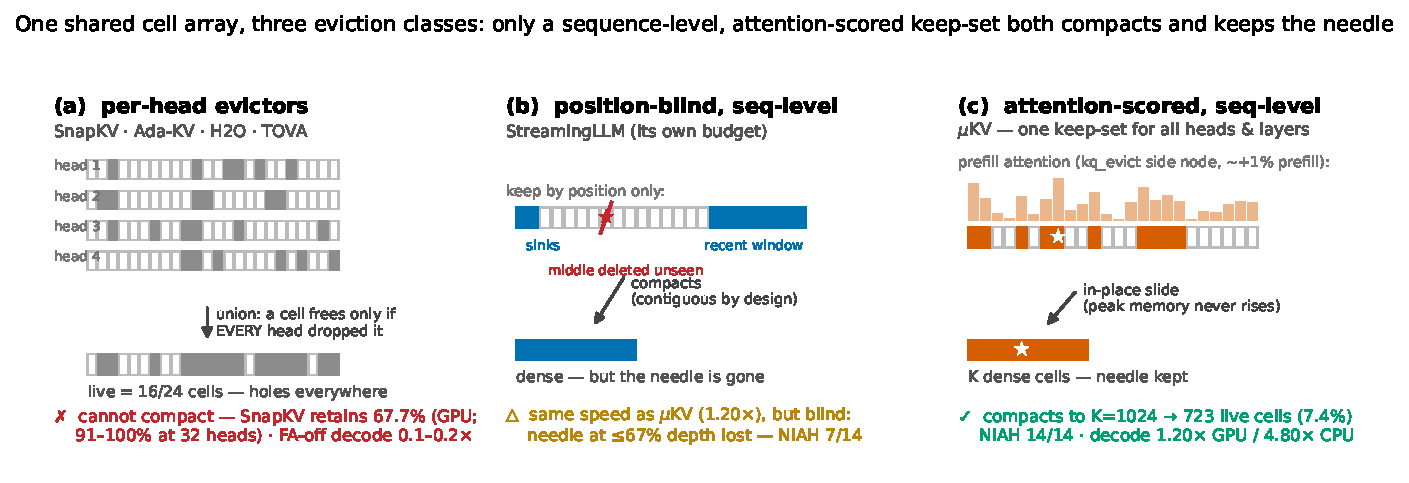
\includegraphics[width=0.79\textwidth]{figures/fig_mechanism_v2.pdf}
\caption{One shared cell array, three eviction classes: \textbf{(a)}~per-head union, \textbf{(b)}~position-blind, \textbf{(c)}~$\mu$KV. Verdict lines are measured.}
\label{fig:mechanism}
\end{figure*}

\section{Introduction}
Long-context LLMs on phones are gated by the KV cache: decode reads it every step, and on a 12--16\,GB device it competes with every foreground app. A rich eviction literature exists (H2O~\cite{h2o}, TOVA~\cite{tova}, SnapKV~\cite{snapkv}, Ada-KV~\cite{adakv}, StreamingLLM~\cite{streamingllm}), all designed and scored on server GPUs. The systems that \emph{do} run on phones move bytes rather than discard them: KVSwap to disk~\cite{kvswap}, DynaKV to UFS~\cite{dynakv}, MobiLoRA across adapters~\cite{mobilora}; none evicts \emph{within} a sequence, none reads the battery.

This paper asks the question the literature skips: \textbf{what actually happens when published eviction policies meet a real phone?} We mean it in end-to-end throughput, energy, temperature, and memory \emph{actually} retained. Prior work stops short: eviction papers evaluate quality on server GPUs (KeyDiff~\cite{keydiff} reports only scoring-kernel latency on a phone), and mobile characterization studies measure energy and thermals without varying the eviction policy. We port nine policies into llama.cpp~\cite{llamacpp}, run each at its \emph{own published configuration} on a OnePlus~15 (Snapdragon 8 Elite Gen 5: CPU, Adreno~840), and measure every axis a deployment decision needs (throughput by phase, perplexity, retrieval, LongBench F1, retained cells, RSS, system energy, temperature) under a cooling and pinned-scheduler discipline we found necessary along the way. Four findings organize the paper:

\begin{enumerate}[leftmargin=*,itemsep=1pt]
\item \textbf{The realizability gap} (\S\ref{sec:break}): published budgets do not materialize on-device. On-device engines keep one cell array shared across heads and layers; a cell is freed only when \emph{every} per-head selector drops it. SnapKV's budget retains 91.3\% of cells on Llama-1B (CPU, FA-on), 94.5\% on Phi-3; H2O's 20\%-of-context ratio retains 94--100\%, so all of them pay eviction's costs and collect none of its benefit.
\item \textbf{The graph split} (\S\ref{sec:break}): the standard implementation route is numerically unsafe on the phone GPU. Intercepting the softmax node forces a scheduler graph split that corrupts the computation on Adreno/Vulkan. In a control on \emph{vanilla}, where nothing is evicted, 10--12.5\% of tokens come out degenerate. Scores must be a \emph{graph output}.
\item \textbf{The KV/W ceiling} (\S\ref{sec:eval}): the model--backend pair, not the policy, decides what eviction is worth. Each decode step reads the weights $W$ and the live cache $\mathrm{KV}$. Eviction shrinks only $\mathrm{KV}$, so no policy beats $(W{+}\mathrm{KV})/W$. On the bandwidth-bound GPU that caps Llama-1B at $1.40\times$; on the CPU, where attention over live cells dominates, the same policy reaches $4.80\times$. A baseline shows it best: KeyDiff is $3.29\times$ on Llama-1B/CPU and $0.27\times$ on Phi-3/GPU, \emph{slower than the full cache}. Eviction papers report speedups without stating the KV/W ratio that sets their own ceiling.
\item \textbf{Compaction feasibility} (\S\ref{sec:design}): the compaction mechanism decides feasibility, not just speed. The state-API round-trip needs a second full context: Phi-3 at 16K is OS-killed on the phone \emph{and} a 24\,GB desktop GPU; in-place sliding compaction runs the same configuration inside prefill's own tensors.
\end{enumerate}

$\mu$KV is the design these findings force (\S\ref{sec:design}): attention-scored like SnapKV, but scored \emph{inside} the FlashAttention graph via a side node (prefill at vanilla parity, 228.5 vs.\ 227.0\,s at a pinned clock, $n{=}3$; FA-off prefill costs $+33$--$111\%$); sequence-level like StreamingLLM, so its budget is realizable and its cache compacts; frozen after prefill; compacted in place. We claim no priority on eviction itself, since KeyDiff~\cite{keydiff} also evicts with FlashAttention intact. \textbf{Our contributions are:} \textbf{(1)} the first end-to-end measurement of published eviction policies on a phone, each at its own configuration, across throughput, energy, temperature, and cells \emph{actually} freed; \textbf{(2)} three mechanisms we identify and quantify that decide whether eviction works there at all: the realizability gap scaling with model width, the graph split, and the KV/W ceiling. Each is a property of the \emph{engine and the device}, not of any policy, which is why we test each on published baselines as well as on $\mu$KV --- a mechanism that only bit our own design would be a bug report, not a finding; \textbf{(3)} $\mu$KV, the design those mechanisms force, with its compaction verified byte-identically and its governor characterised as a measured dial; and \textbf{(4)} the measurement traps that make on-device eviction numbers wrong, quantified: a baseline at the wrong budget reads $5.75$ rather than $29.07$\,tok/s, and an unpinned scheduler spreads identical runs by $39\%$ (\S\ref{sec:eval}).

\section{Three ways the phone breaks the literature}
\label{sec:break}


\textbf{Realizability.} llama.cpp stores KV in one cell array indexed by position; other mobile engines page it in blocks (MLC) or keep per-layer tensors, but in every on-device engine we know of the unit of storage \emph{spans all KV heads}. A per-head policy hands the engine $H{\times}L$ different keep-sets; the engine can free only the intersection of their complements (Fig.~\ref{fig:mechanism}a). KV-Compress~\cite{kvcompress} notes this for server layouts, and AhaKV~\cite{ahakv} keeps attention scoring \emph{with} FlashAttention on yet still selects \emph{per head}, claiming low-resource benefit it never tests on a device; we quantify it on-device, where unanimity gets rarer as heads multiply. Measured on one build at published budgets: at Llama-1B's 8 KV heads the per-head class still spreads (Ada-KV retains 35.8\%, TOVA 42.0\%, SnapKV 91.3\%), but at Phi-3's 32 heads all of them collapse into an 85--100\% band (Ada-KV 94.0\%, SnapKV 94.5\%, H2O 100.0\%: 20.4M eviction attempts freeing zero cells), and their throughputs converge to $1.38$--$1.42\times$. $\mu$KV's 14/14 reproduces on CPU for Phi-3 (17\% retained) and Bonsai-8B (18\%). Sequence-level selection is immune by construction: across the same width change $\mu$KV holds 7.4\% to 12.3\% and StreamingLLM ${\sim}$20 to 26\%; $\mu$KV still evicts on gemma-2's interleaved-SWA cache (715 cells, $2.4\times$) where KeyDiff's eviction never fires at all (0 evicted, 5674 of 5674 retained, $1.02\times$), but that layout is also the one place in-place compaction declines (\S\ref{sec:design}). A budget is only as real as the cache layout lets it be, and so is a compaction. As models widen, per-head eviction on shared-cell engines trends toward a no-op that costs energy: every Phi-3 per-head cell burns \emph{more} than the full cache. This is invisible in a server evaluation with per-head paged storage and decisive on a phone: \emph{retained cells}, not nominal budget, set the bandwidth and the memory.

\textbf{The graph split.} The standard way to read attention scores in a graph engine is an eval-callback on the softmax node. On Adreno/Vulkan every FA-off policy's output is corrupted, 1--13\% of tokens depending on the policy, while vanilla FA-off is clean, vanilla being the one configuration that installs no callback. A three-way control isolates it: no callback 0/978 degenerate, callback reading the tensor 76/609, callback \emph{requesting but never reading} 68/679. The cause is execution granularity: a callback makes the scheduler run the split as separate \texttt{ggml\_graph\_view} fragments, chunked where it is \emph{asked} for a node, before any read; that path is correct on the CPU backend and only wrong on this one. Retrieval confirms it across backends: FA-off policies find the needle on the CPU (H2O 8/14, TOVA 12/14) and collapse on Adreno (3/14, 2/14); FA-on policies are unchanged. The fix is structural: scores must be a node the graph \emph{produces} ($\mu$KV's side node) rather than an interception of one it consumes. Our build now enforces this: on unsafe geometries it auto-promotes prefill-time policies to the side node and refuses per-step ones, recording the verdict in every cell's metadata (Table~\ref{tab:gpu}).

\textbf{The roofline, and why it is a GPU statement only.} Per decode token the device reads the weights $W$ plus the live cache. Llama-3.2-1B is heavily GQA-compressed (8~KV heads $\times$ 64 dims $=$ 32\,KB/cell): its cache at the 9.7K prompt is 304\,MB against 770\,MB of weights, so on the \emph{bandwidth-bound GPU} a \emph{zero-size} cache caps any evictor at $1.40\times$, so two policies that both reach ${\sim}2$k cells are indistinguishable by construction, which is exactly what we measure ($\mu$KV 29.05, StreamingLLM 29.07\,tok/s). Phi-3 (32 heads $\times$ 96 dims, $12\times$ the bytes per cell) has KV/W$=1.83$, a $2.83\times$ ceiling, and measures $2.64\times$ prompt-matched on one build.

\textbf{On the CPU the same arithmetic does not apply, and the lever inverts.} Vanilla decodes at 5.02\,tok/s, five times slower than its own weight-bandwidth bound, so the binding resource is not bytes but \emph{attention compute over live cells}. Going $9741\!\rightarrow\!721$ cells is $\mathbf{4.80\times}$, far above the $1.34\times$ a bandwidth model predicts. \emph{The same policy at the same budget is decisive on one processor and nearly irrelevant on the other.}

\textbf{A second factor, independent of budget: the execution path.} Fig.~\ref{fig:stalls} plots what the cache does \emph{not} explain. Across nine policies, deep-throttle residency correlates $r{=}{+}0.94$ with whether FlashAttention is off and $r{=}{-}0.12$ with cache size; \texttt{psi\_io} is 0.000 and 6.6--7.2\,GB stay free at every point, so no memory-pressure path exists. StreamingLLM and $\mu$KV read an \emph{identical} 823\,MB/token (777 vs.\ 721 cells) and differ $3.6\times$ in throughput purely on FA on/off. Normalised by work done, $\mu$KV has the \emph{lowest} throttle exposure of every policy measured (13\,s per 1000 tokens against vanilla's 31 and the FA-off cluster's 85--106): it finishes the same 4096 tokens in a fifth of the time, so an equal \emph{fraction} of a shorter run is far less absolute exposure.

\section{$\mu$KV}
\label{sec:design}

\begin{figure*}[t]
\centering
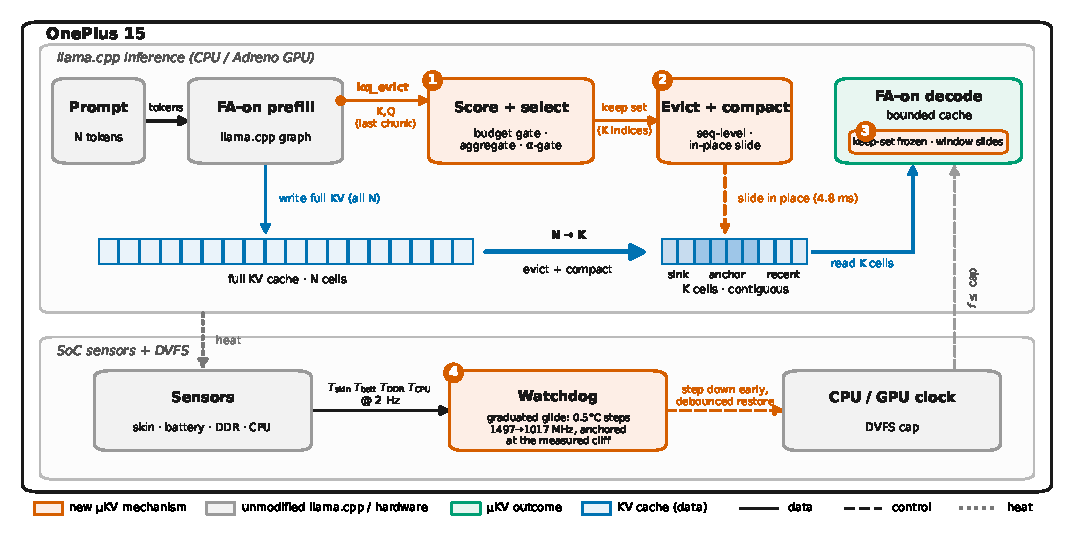
\includegraphics[width=0.55\textwidth]{figures/fig_architecture_v6.pdf}
\caption{$\mu$KV's pass: in-graph scoring, one keep-set for all heads, in-place compaction. The thermal loop never touches the keep-set.}
\label{fig:arch}
\end{figure*}

Mechanically, $\mu$KV is four decisions (Fig.~\ref{fig:arch}), each forced by \S\ref{sec:break}: \textbf{(i)} score in-graph (side node, FA never off); \textbf{(ii)} select once at end of prefill, at sequence level. \emph{$K$ itself does not adapt} --- it is 1024 in every number in this paper; what adapts is how $K$ is spent. Writing $\bar a_p$ for the attention mass at position $p$ averaged over layers, heads and queries, and treating the last $R_{\min}{=}32$ tokens as the recent region, the $\alpha$-gate sets $\alpha_a=\sum_{p<N-R_{\min}}\bar a_p / \sum_p \bar a_p$, clipped to $[0.05,0.95]$ and floored at 0.70, then splits the budget as $n_{\text{anchor}}{=}\alpha_a(K{-}\text{sinks})$ and $n_{\text{recent}}$ the remainder. A per-head gate sizes each head's share from its own attention concentration (crediting Ada-KV~\cite{adakv} for the per-head idea), but the emitted keep-set is one set for all heads and layers. The floor is the one tuned constant: on retrieval prompts $\alpha_a$ collapses toward 0.54 and starves the anchors, while on the WikiText prompt it is not binding ($\alpha_a{=}0.707$ measured); \textbf{(iii)} freeze during decode (only the recent window slides); \textbf{(iv)} compact in place. \textbf{$\mu$KV's prefill overhead is a property of the clock, not of the policy.} Protocol, not policy, sets prefill here: the same vanilla configuration spans 172--537\,s across protocols, so cross-campaign prefill comparisons are meaningless. Cool-gated from cold (Table~\ref{tab:cpu}'s protocol) $\mu$KV costs $+13.7\%$ (vanilla $182{\pm}7$\,s vs.\ $207{\pm}11$); warmed, every arm lands in one 240--249\,s band. Four attempts to separate the two by matching \emph{temperature} failed, because the cores shed a busy-loop's heat within a second of the load stopping. So we matched the \emph{clock} instead (governor pinned at 1632\,MHz, verified throughout each run), and the disagreement disappears: vanilla $227.0{\pm}1.5$\,s, $\mu$KV $228.5{\pm}2.9$, StreamingLLM $227.4{\pm}1.0$ ($n{=}3$, rotated). \emph{At a fixed clock the entire policy effect is $+0.7\%$}, and the $2.7\times$ spread we had been reading as a policy difference was governor state. That is what one side node on the last chunk costs; emitting it on every chunk instead cost $+106\%$.

\textbf{Parameters, and how they were not chosen.} The full shipped config is $K{=}1024$, 4 sinks, observation window 16, SnapKV pool 7, adaptive anchor with $r_{\min}{=}32$, $\alpha$-gate floor 0.70. \emph{This one string produced every $\mu$KV number in this paper} --- four models, two backends, three benchmarks --- and was never re-tuned per model, per task, or per device. Nothing is fitted to an evaluation set: the K sweep that motivated 1024 ran on a different model (Bonsai-8B) and the smallest budget was also the best there, so the choice costs nothing to defend. Compaction is verified at the task level, holding the keep-set identical to the cell (13--21K dropped per run) so compaction is the only variable, and comparing generated text byte for byte. \textbf{In-place} sliding is output-preserving: 23 of 25 pairs byte-identical across Llama-3.2-1B, Phi-3 and Bonsai-8B, 24 of 25 on the answer span, the two exceptions being a trailing period and post-answer commentary. Perplexity locates the perturbation: across the 23 byte-identical pairs it still moves, by a median of 0.20\% and never above 1.69\%, so compaction does shift the logits --- a compacted cache reduces in a different order --- but never past an argmax boundary. That is the mechanism: survivors keep their positions and 2D extents under a slide, so RoPE is unchanged, and a rebuild has no such guarantee. We cannot yet put a number on the \textbf{round-trip}: it engages only where in-place declines, which on our models is gemma-2's interleaved-SWA cache alone, and gemma-2's 8192-token window is shorter than these prompts, so both arms degenerate and neither certifies the other. Its cost we can state --- a second full context, which is what the OS kills.


\begin{figure*}[t]
\centering
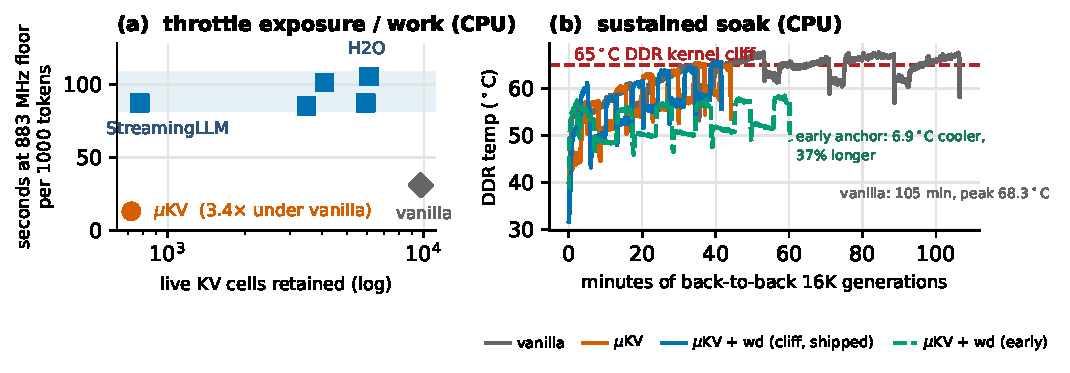
\includegraphics[width=0.72\textwidth]{figures/fig_throttle_v2.pdf}
\caption{\textbf{(a)}~Throttle exposure per 1000 decoded tokens, seconds at the 883\,MHz floor. \textbf{(b)}~Six-generation soak, one cool gate then none.}
\label{fig:stalls}
\end{figure*}

\section{Evaluation}
\label{sec:eval}
\textbf{Setup and discipline.} OnePlus 15; llama.cpp, one build per table; f16 KV (q8\_0 is numerically broken on this Adreno driver); Phi-3-mini-128k; every baseline at its own published configuration: SnapKV window~32/pool~7, Ada-KV 2048, TOVA 2048, H2O 20\%-of-$N$ resolved per prompt, StreamingLLM \texttt{start\_size}~4 $+$ \texttt{recent\_size}~2000~$=$~2004 from its repository defaults. Timed cells: cool-gated (DDR$\le$35, battery$\le$33, cores$\le$45$^\circ$C; charging off), scheduler-pinned. Pinning matters: unpinned, identical GPU runs spread 28.2--39.2\,tok/s (scheduler, not thermal); pinning collapses that to 3\%, so any phone-GPU ratio below $1.39\times$ published without it is inside the noise. Energy: USB rail $+$ coulomb counter. Our own earlier comparisons failed this bar and are corrected here. StreamingLLM had run FA-off, uncompacted, at half budget (5.75 vs.\ faithful 29.07\,tok/s); its implementation compacts on every eviction, so compaction is intrinsic to it.




\begin{table}[t]
\caption{\textbf{Sustained decode, phone CPU.} 9.7K prompt $+$ 4K decode, Llama-3.2-1B Q4\_K\_M, 6 threads. $^{*}$$n{=}3$, Latin-square, mean$\pm$SD. \emph{Italic}: budget never materialised.}
\label{tab:cpu}
\scriptsize
\setlength{\tabcolsep}{2.6pt}
\begin{tabular}{llrrrrr}
\toprule
\textbf{Policy} & \textbf{Config} & \textbf{tok/s} & \textbf{$\times$van} & \textbf{Wall\,(s)} & \textbf{mWh} & \textbf{ActKV} \\
\midrule
\textbf{$\mu$KV}$^{*}$ & K=1024 & $\mathbf{23.91{\pm}0.37}$ & \textbf{4.80} & \textbf{379} & \textbf{595} & \textbf{721} \\
KeyDiff$^{*}$      & K=2048 & $16.40{\pm}0.11$ & 3.29 & 484 & 700 & 2049 \\
Ada-KV             & FA \textbf{on} & 11.52 & 2.29 & 566 & 845 & 3489 \\
StreamingLLM$^{*}$ & 4+2000 & $10.25{\pm}0.06$ & 2.06 & 580 & 781 & 2001 \\
SnapKV             & FA off & 6.83 & 1.36 & 849 & 1180 & 5931 \\
Ada-KV             & FA off & 6.79 & 1.35 & 856 & 1194 & 3485 \\
KeyDiff            & K=8192 & 6.43 & 1.28 & 812 & 1261 & 8195 \\
H2O                & FA off & 6.45 & 1.29 & 856 & 1262 & \textit{9151} \\
TOVA               & FA off & 5.92 & 1.18 & 917 & 1200 & 4093 \\
SnapKV             & FA \textbf{on} & 5.38 & 1.07 & 953 & 1346 & \textit{8893} \\
vanilla$^{*}$      & full cache & $4.99{\pm}0.01$ & 1.00 & 1004 & 1431 & 9741 \\
\midrule
\multicolumn{7}{l}{\emph{$\mu$KV on the other CPU models, same protocol, each vs.\ its own vanilla:}}\\
Phi-3-mini   & K=1024 & 5.53 & 4.54 & 841 & 928 & 929 \\
Bonsai-8B (1-bit) & K=1024 & 4.46 & 4.43 & 1996 & 2415 & 789 \\
\quad\emph{vs.\ KeyDiff} & K=2048 & 2.01 & 2.00 & --- & --- & 2048 \\
gemma-2-2b (iSWA) & K=1024 & 9.28 & 2.40 & --- & --- & 715 \\
\bottomrule
\end{tabular}
\end{table}

\begin{table}[t]
\caption{\textbf{Phone GPU.} 12K prompt $+$ 4K decode; Llama rows $n{=}3$. Every generation is text-graded. On Phi-3 the gate promotes SnapKV and Ada-KV and refuses H2O and TOVA (\S\ref{sec:break}).}
\label{tab:gpu}
\scriptsize
\setlength{\tabcolsep}{3pt}
\begin{tabular}{lrrrr}
\toprule
\textbf{Policy} & \textbf{tok/s} & \textbf{vs van.} & \textbf{mWh} & \textbf{Cells} \\
\midrule
vanilla                & $24.28{\pm}0.12$ & $1.00\times$ & 437 & 9741 \\
\textbf{$\mu$KV}       & $\mathbf{29.05{\pm}0.13}$ & $1.20\times$ & \textbf{400} & \textbf{723} \\
StreamingLLM           & $29.07{\pm}0.18$ & $1.20\times$ & 401 & 2005 \\
per-head (4) / KeyDiff & 2.9--4.8 / 1.6 & 0.11--0.19$\times$ / 0.06$\times$ & --- & 2049--6592 \\
\midrule
\multicolumn{5}{l}{\emph{Phi-3-mini block (KV/W$=1.83$); compare \textbf{within} a block only:}}\\
vanilla                & 5.05 & $1.00\times$ & 1936 & 11157 \\
\quad\textbf{$\mu$KV (in-place)} & \textbf{13.36} & $\mathbf{2.64\times}$ & \textbf{1186} & \textbf{878} \\
\quad StreamingLLM & 10.60 & $2.10\times$ & 1126 & 2000 \\
\quad Ada-KV (promoted) & 9.13 & $1.81\times$ & 1430 & 4326 \\
\quad SnapKV (promoted) & 5.80 & $1.15\times$ & 1837 & \textit{10862} \\
\quad KeyDiff (2K)      & 1.36 & $0.27\times$ & 2402 & 2048 \\
\quad H2O / TOVA        & \multicolumn{4}{c}{refused by gate: FA-off capture corrupt at head\_dim 96} \\
\bottomrule
\end{tabular}
\end{table}

\textbf{Speed and energy.} Table~\ref{tab:cpu}. $\mu$KV reaches $4.80{\pm}0.07\times$ vanilla on 721 live cells at 595\,mWh ($-58\%$); the best baseline, KeyDiff at its smallest published budget, is $1.46\times$ slower on $2.8\times$ the cells and $18\%$ more energy. The margin survives sustained use: six back-to-back 16K generations with no cooling hold $\mu$KV at $23.0$--$23.3$\,tok/s (\S\ref{sec:disc}), so the speedup is not a cold-start artefact. Two baselines were previously handicapped by our harness and are corrected here: Ada-KV scored from the in-graph side node with its own window runs $1.70\times$ faster than through the FA-off capture (11.52 vs.\ 6.79) at identical retention, while SnapKV runs \emph{slower} FA-on (5.38 vs.\ 6.83) and retains more (8893 vs.\ 5931 cells), its windowed scores yielding a larger per-head union. We report both configurations rather than the flattering one.

\begin{table}[t]
\caption{\textbf{Quality at each policy's own published budget} (LongBench token-F1, $n{=}15$). Retention sits beside every score; \emph{italic} marks a budget that never materialised.}
\label{tab:quality}
\small
\setlength{\tabcolsep}{4pt}
\begin{tabular}{lcccc}
\toprule
 & \multicolumn{2}{c}{\textbf{qasper}} & \multicolumn{2}{c}{\textbf{hotpotqa}} \\
\cmidrule(lr){2-3}\cmidrule(lr){4-5}
\textbf{Policy} & F1 & retained & F1 & retained \\
\midrule
vanilla (full cache)   & 20.29 & 100\% & 36.00 & 100\% \\
\textbf{$\mu$KV} (K=1024) & 17.32 & \textbf{18.2\%} & \textbf{29.79} & \textbf{13.7\%} \\
KeyDiff 8K$^{\S}$      & ---   & ---   & \textbf{36.39} & 62.3\% \\
KeyDiff 6K$^{\S}$      & ---   & ---   & 29.33 & 48.4\% \\
KeyDiff 2K             & 23.46 & 47.6\% & 15.84 & 20.0\% \\
StreamingLLM$^\dagger$ & 19.31 & 46.5\% & 23.57 & 19.5\% \\
SnapKV                 & 20.05 & \textit{97.0\%} & 40.00 & \textit{89.1\%} \\
Ada-KV                 & 20.05 & \textit{85.7\%} & 40.00 & \textit{53.7\%} \\
H2O                    & 17.84 & \textit{91.5\%} & 39.79 & \textit{91.8\%} \\
TOVA                   & 20.05 & \textit{91.2\%} & 39.89 & \textit{57.4\%} \\
\bottomrule
\end{tabular}
\end{table}




\begin{table}[t]
\caption{\textbf{Retrieval, phone GPU.} 14 stimuli $\times$ 7 depths, retention beside every score. \emph{Italic}: budget never materialised. $^{\ddagger}$FA-off, invalid on this backend (\S\ref{sec:break}).}
\label{tab:niah}
\small
\setlength{\tabcolsep}{5pt}
\begin{tabular}{lcccc}
\toprule
\textbf{Policy} & \textbf{Budget} & \textbf{NIAH} & \multicolumn{2}{c}{\textbf{Retained 4K / 8K}} \\
\midrule
vanilla                & ---  & 14/14 & 100\% & 100\% \\
\textbf{$\mu$KV}       & 1024 & \textbf{14/14} & \textbf{25.2\%} & \textbf{13.0\%} \\
KeyDiff                & 2048 & 14/14 & 65.6\% & 33.6\% \\
KeyDiff$^{\S}$         & 6144 & 14/14 & 100\% & 100\% \\
Ada-KV                 & 1024 & 12/14 & \textit{76.9\%} & \textit{52.2\%} \\
SnapKV                 & 1024 & 12/14 & \textit{100\%} & \textit{98.2\%} \\
StreamingLLM$^\dagger$ & 2004 & 7/14 & 64.2\% & 32.9\% \\
H2O$^{\ddagger}$       & 1024 & 3/14 & \textit{100\%} & \textit{99.3\%} \\
TOVA$^{\ddagger}$      & 1024 & 2/14 & \textit{85.2\%} & \textit{60.7\%} \\
\bottomrule
\end{tabular}
\end{table}

\textbf{Quality, read with retention} (Table~\ref{tab:quality}). Per-head policies appear to win (SnapKV 40.00 on hotpotqa vs.\ $\mu$KV's 29.79) while retaining 89.1\% of the cache; six of their fifteen generations are \emph{byte-identical to vanilla's}: the realizability gap reappearing on the quality axis.

\textbf{KeyDiff at its own published budgets} splits. Its 8K claim reproduces: 36.39 F1 vs.\ a 36.00 full cache ($+1.1\%$; claim $\le0.04\%$), retaining 62.3\%. Its 6K claim does not survive our prompt lengths: 29.33 F1, $-18.5\%$ vs.\ a claimed $\le1.5\%$, because hotpotqa's median prompt is 15.5K tokens, so 6144 cells retain only 48\%, far harsher than the LongBench average behind their number. The comparison that matters: \textbf{$\mu$KV reaches 29.79\,F1 on 1763 live cells where KeyDiff-6K reaches 29.33 on 5886}, equal quality on $3.3\times$ less cache; KeyDiff needs 62\% retention to match full where $\mu$KV delivers 83\% of it at 13.7\%.

\textbf{The pattern is not a phone artefact.} Repeating hotpotqa on an RTX~4500 ($n{=}50$) reproduces it: per-head policies retain 33--81\% there too (shared cell array on every backend; vanilla 42.14\,F1, SnapKV 41.12 at 80.8\%). At \textbf{8.7\%} retention $\mu$KV scores 40.72, within 1.4\,F1 of full, while StreamingLLM, the only other policy in that retention class, loses 8.8\,F1. On qasper six policies \emph{beat} the full cache (distractor filtering, \S\ref{sec:disc}), so qasper cannot rank eviction quality and we do not use it to.

\textbf{Why the cache at all: the privileged-lever boundary.} Three actuators cut decode energy here, measured under one protocol, and the ranking that matters is \emph{reachability}, not effect size. Capping the GPU clock is the strongest thermal lever, since 1200$\to$902\,MHz costs no throughput (30.0 vs.\ 30.3\,tok/s: decode is bandwidth-bound, so the clock is idle headroom) and drops peak DDR $16.6^\circ$C, but it is a write to \texttt{/sys/class/kgsl/\allowbreak kgsl-3d0/max\_gpuclk}; scheduler pinning removes a 39\% dispatch bimodality but needs \texttt{nice -20}. \textbf{Both require root; an application can reach neither.} KV-cache size is the only actuator inside the inference engine. It is the weakest of the three, the only one that costs quality, and the only one that makes the device \emph{hotter} (k-pct~10 runs $5.8^\circ$C above k-pct~20). It is also the only one a runtime may use, which is why a battery-aware cache policy is worth building, and why its tiers must come from a measured frontier rather than chosen thresholds.

\textbf{The frontier, and what it refuted.} A controller reads state-of-charge and sets $K$ as a fraction of prompt length ($K{=}1947/974/487$, $n{=}3$ rotated). Quality per tier ($n{=}15$): qasper 17.5/10.9/10.6 vs.\ 20.3 full; hotpotqa flat at 29.8 vs.\ 36.0, so the price of a tier step is task-dependent, zero on factoid QA, $-6.7$\,F1 on multi-fact QA. The 5\% rung is dominated and deleted. 

\textbf{But the lever itself does not survive its own test.} We re-ran the ladder cooled, scheduler-pinned and interleaved ($n{=}3$) with the GPU clock held at 902\,MHz, so that cache budget is the \emph{only} variable. Halving the cache ($K{=}1947\!\rightarrow\!974$, 1379$\rightarrow$688 live cells) changes decode energy by $\mathbf{+1.0\%}$, inside the 8--10\% run-to-run spread of both arms, while buying $+13.1$\% throughput, costing $+3.5^\circ$C, and costing 6.7\,F1. \emph{On the phone GPU the cache tier is not an energy actuator at all.} A battery-aware controller that shrinks the cache gives up quality and runs hotter for no energy return. 

\textbf{The regime decides, and the controller reads the wrong variable.} On the CPU, where decode is attention-bound over live cells, $9741\!\rightarrow\!721$ cells is $-61$\% energy (601 vs.\ 1544\,mWh); on the GPU, where 800\,MB of weights dominate 45\,MB of cache, the same reduction is worth nothing. KV/W tells you which regime you are in, and our controller, as built, \emph{adapts on the GPU} (1379/688/342 cells) and \emph{declines on the CPU} (341 cells at every battery level), which is exactly backwards. The corrected design conditions on KV/W, not on the battery alone. We report this as a negative result rather than repair it silently: it is the clearest evidence in this paper that a lever's value is a property of the model--backend pair and not of the policy.

\begin{table}[t]
\caption{\textbf{Governor, phone CPU soak.} Six generations, one cool gate then none. \emph{Anchor} is the battery temperature at which the ladder's first step fires.}
\label{tab:gov}
\small
\setlength{\tabcolsep}{4.5pt}
\begin{tabular}{lccccc}
\toprule
\textbf{Run} & \textbf{Anchor} & \textbf{Gen 1} & \textbf{Steady} & \textbf{Floor} & \textbf{Peak} \\
 & ($^\circ$C) & (tok/s) & (tok/s) & (\%) & DDR \\
\midrule
vanilla          & ---  & 4.97  & 4.99  & 3.3 & 68.3 \\
vanilla          & 47   & 5.01  & 4.98  & 3.6 & 67.2 \\
\midrule
$\mu$KV          & ---  & 23.32 & 23.14 & 8.2 & 65.6 \\
\textbf{$\mu$KV} & \textbf{47} & \textbf{26.95} & 22.97 & \textbf{6.4} & 66.0 \\
$\mu$KV          & 42   & 27.12 & 21.07 & 5.4 & 63.3 \\
$\mu$KV          & 35   & 18.00 & 15.95 & 2.4 & 58.7 \\
\bottomrule
\end{tabular}
\end{table}

\section{Discussion: negatives and open problems}
\label{sec:disc}
HotMobile asks what did \emph{not} work; each item is a measurement. \textbf{Cache moves heat only where it moves traffic:} halving the cache at a held GPU clock raises \emph{peak} DDR $5.8^\circ$C (mean $+2.3$), the freed bandwidth becoming work; but on the CPU at unforced-equal clock (1374 vs.\ 1378\,MHz) $\mu$KV is $2.4^\circ$C \emph{cooler} on DDR at $4.6\times$ throughput. The sign is set by the backend. \textbf{The watchdog buys clock while the device is cool, not while it is hot} (Table~\ref{tab:gov}). The vendor gives a cliff: flat 1498\,MHz from 46--49$^\circ$C, then 883 at 50.0. Ours replaces it with a staircase (0.5$^\circ$C steps, 1497$\to$1017\,MHz, immediate-up/debounced-down). The gain is \emph{front-loaded} and \emph{conditional on the workload}: $\mu$KV's cool generation gains $+15.5\%$, because at tier~0 it writes \texttt{cpuinfo\_max\_freq}, releasing a ceiling the vendor HAL had already lowered. On vanilla it gains $+0.9\%$: that run is bandwidth-bound and cannot spend released clock, so the headroom returns as temperature ($-2.4^\circ$C mean DDR). \emph{The governor converts headroom into whichever resource the workload lacks}, so it needs eviction to appear as speed. Both $\mu$KV arms then converge to ${\sim}1378$\,MHz, so the watchdog is free rather than a sustained win. The ladder is weak \emph{by construction}: over 883--1632\,MHz CPU power is \emph{linear} in clock ($f^{0.97}$, $R^2{=}0.99$), so voltage never moves and a step buys ${\sim}7\%$ power, not the ${\sim}20\%$ voltage scaling would give. The anchor is a monotone dial whose sign depends on the backend: earlier trades throughput for temperature on the CPU (Table~\ref{tab:gov}); on the GPU its ends trade different currencies: the early anchor (36$^\circ$C) \emph{gains} $+10.8\%$ (residency $41.0\!\to\!37.0\%$), the late one (47$^\circ$C) buys residency $41.0\!\to\!28.5\%$ for $+0.8\%$. \textbf{Peak RSS rises under eviction} (the engine allocates the full context up front): the win is retained cells and bandwidth, not peak footprint. \textbf{Perplexity cannot referee eviction:} on a disjoint slice every evictor we can score \emph{beats} the full cache ($\mu$KV 22.7 vs.\ 23.5): PPL certifies harmlessness; only retrieval/QA separate policies.

\textbf{Future work, for this workshop to argue about.} (1) \emph{Scores as graph outputs}: the split of \S\ref{sec:break} makes callback scoring unsafe, and per-head paging (shipping server-side) is not on phones yet; the head-count law quantifies what it must fix. (2) Phase-aware DVFS exists for servers; no \emph{shipped} mobile governor knows the runtime's phase, a gap worth a measured $16.6^\circ$C of free headroom. (3) Offloading (KVSwap, DynaKV) and eviction should be \emph{composed}: offloaders write the whole cache and select at recall, where an evictor's scores can triage at \emph{write} time (keep/park/discard).

\begin{thebibliography}{9}
\scriptsize\setlength{\itemsep}{-3pt}\setlength{\parskip}{0pt}
\bibitem{h2o} Z.~Zhang et al. H2O. \emph{NeurIPS}, 2023.
\bibitem{tova} M.~Oren et al. TOVA: Transformers are multi-state RNNs. \emph{EMNLP}, 2024.
\bibitem{snapkv} Y.~Li et al. SnapKV. \emph{NeurIPS}, 2024.
\bibitem{adakv} Y.~Feng et al. Ada-KV. \emph{NeurIPS}, 2025.
\bibitem{streamingllm} G.~Xiao et al. Efficient streaming LMs with attention sinks. \emph{ICLR}, 2024.
\bibitem{keydiff} J.~Park et al. KeyDiff: Key similarity-based KV cache eviction. \emph{NeurIPS}, 2025. arXiv:2504.15364.
\bibitem{ahakv} Y.~Gu et al. AhaKV: Attention-driven KV cache eviction. arXiv:2506.03762, 2025.
\bibitem{kvcompress} I.~Rehg. KV-Compress. arXiv:2410.00161, 2024.
\bibitem{kvswap} H.~Zhang, C.~Xia, Z.~Wang. KVSwap: Disk-aware KV cache offloading on-device. \emph{MobiSys}, 2026.
\bibitem{dynakv} T.~Wang et al. DynaKV: Long-sequence LLM decoding on smartphones. arXiv:2511.07427, 2025.
\bibitem{mobilora} B.~Li et al. MobiLoRA: Context-aware KV cache optimization for mobile LoRA inference. \emph{ACL}, 2025.
\bibitem{llamacpp} G.~Gerganov et al. llama.cpp (github.com/ggml-org).
\end{thebibliography}

\end{document}
